\newSection{Related Works}

\subsection{HairNet}
\begin{frame}\frametitle{Related Works}
    \framesubtitle{HairNet}

    \normalsize{\textcolor{myBlue}{\emph{Single-View Hair Reconstruction using Convolutional Neural Networks}}}
    
    \begin{figure}[ht]
        \centering
        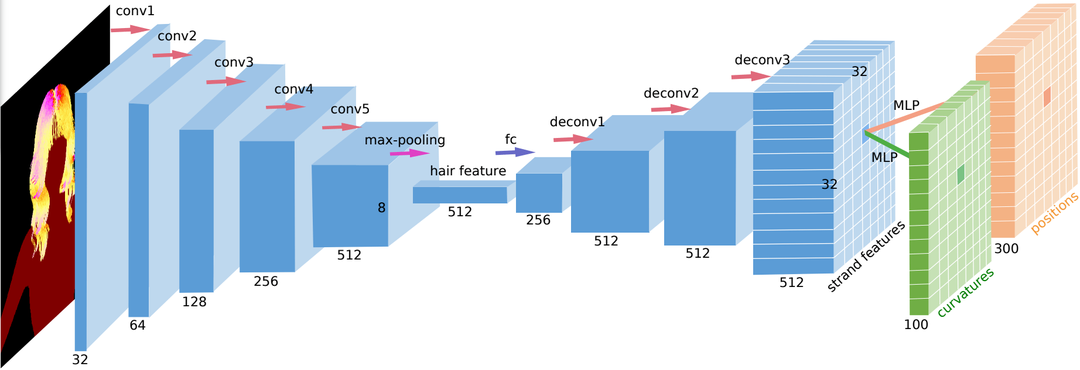
\includegraphics[width=0.8\linewidth]{assets/figures/baselines/HairNet.png}
        \caption{Zhou et al. 2018\cite{Zhou2018SingleViewHR}}
        \label{fig:hairnet}
    \end{figure}
\end{frame}


\subsection{3D Hair Synthesis}
\begin{frame}\frametitle{Related Works}
    \framesubtitle{3D Hair Synthesis}

    \normalsize{\textcolor{myBlue}{\emph{3D Hair Synthesis using Volumetric Variational Autoencoders}}}
    
    \begin{figure}[ht]
        \centering
        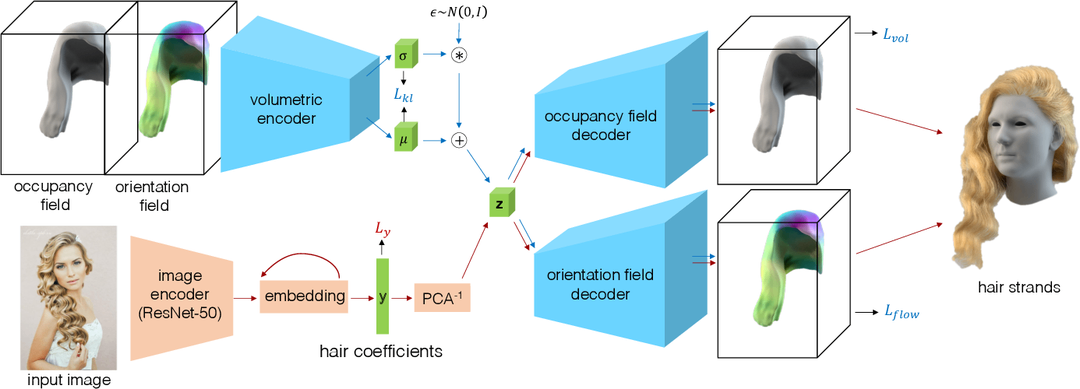
\includegraphics[width=0.8\linewidth]{assets/figures/baselines/3DHairSynthesis.png}
        \caption{Saito et al. 2018\cite{Saito20183DHS}}
        \label{fig:3dhairsynthesis}
    \end{figure}
\end{frame}


\subsection{NeuralHDHair}
\begin{frame}\frametitle{Related Works}
    \framesubtitle{NeuralHDHair}

    \normalsize{\textcolor{myBlue}{\emph{NeuralHDHair: Automatic High-fidelity Hair Modeling from a Single Image Using Implicit Neural Representations}}}
    
    \begin{figure}[ht]
        \centering
        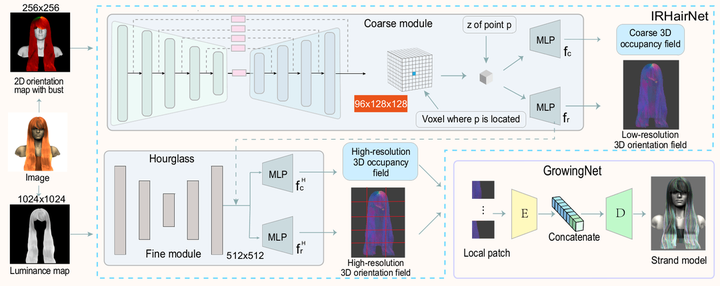
\includegraphics[width=0.8\linewidth]{assets/figures/baselines/NeuralHDHair.png}
        \caption{Wu et al. 2022\cite{wu2022neuralhdhair}}
        \label{fig:neuralhdhair}
    \end{figure}
\end{frame}

